This chapter describes an experiment that will compare the various implemented cache partitioning algorithms both against \gls{lru} and against each other.
When executing this experiment, we utilize the base system configuration as previously detailed in Table~\ref{tbl:processor_model:properties}.
The L2 cache size is set to 128kB per core, and the L3 cache size is set to 4MB, 8MB or 16MB for respectively 4-, 8- and 16-core workloads.
Each workload is simulated until all benchmarks in that workload have completed at least once. 
The first time a benchmark completes we store its statistics.
After completion, a benchmark will be restarted unless it is the last benchmark to complete in which case we end the workload.
We generate reference statistics for each benchmark by executing it in private mode.
In private mode, we use the same system as in this experiment but with only a single core, the L2 and L3 sizes are set equal to the 4-core workloads; 128kB L2 and 4MB L3.

This chapter is divided into three sections.
In the first section, we present average algorithm performance by core count.
Next, we then take a closer look at the results of the five 4-core workload groups.
The final section covers the performance of cabw workloads.

\section{Overall Results}
\label{sec:results:cache_partition}

\begin{figure}[th]
    \centering
    \begin{subfigure}[b]{0.5\textwidth}
        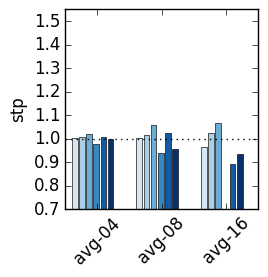
\includegraphics[width=.8\textwidth]{figures/results/speedup/avg-stp-0128k-0100-avg}
        \caption{STP (not shown; \gls{pipp} 0.55).}
        \label{fig:results:base:avg:stp}
    \end{subfigure}%
    \begin{subfigure}[b]{0.5\textwidth}
        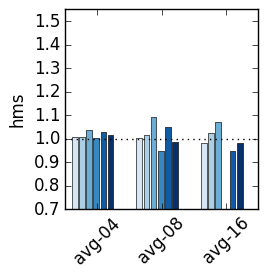
\includegraphics[width=.8\textwidth]{figures/results/speedup/avg-hms-0128k-0100-avg}
        \caption{HMS (not shown; \gls{pipp} 0.61).}
        \label{fig:results:base:avg:hms}
    \end{subfigure}
    \begin{subfigure}[b]{0.5\textwidth}
        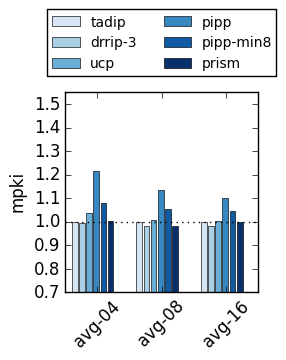
\includegraphics[width=.8\textwidth]{figures/results/speedup/avg-mpki-0128k-0100-avg}
        \caption{MPKI}
        \label{fig:results:base:avg:mpki}
    \end{subfigure}
    \caption[Average result grouped by core]{Average \gls{stp}, \gls{hms} and \gls{mpki} normalized to \gls{lru} for all workloads, grouped by number of cores.}
    \label{fig:results:base:avg}
\end{figure}



Figure~\ref{fig:results:base:avg:stp} shows the average speedup of all workloads normalized to \gls{lru} performance grouped by workload size.
We observe that most of the implemented algorithms perform close to \gls{lru} for the four core workloads.
\gls{ucp} gives the best speedup of 2.1\% while \gls{pipp} performs badly with a 2.4\% performance decrease. 
The modified version of \gls{pipp}, PIPP-min8, performs as good as \gls{lru}.
When considering the harmonic mean of speedups as shown in Figure~\ref{fig:results:base:avg:hms} we observe that all algorithms perform as good or better than \gls{lru}.  
Most noticeable is \gls{pipp}, which in terms of \gls{hms} is equal to \gls{lru}.
As explained in Section~\ref{sec:methodology:metrics}, \gls{stp}  is a measure of the overall speedup of all benchmarks in the workload, and a decrease indicates that completing all of them is slower.
\gls{hms}, however, measures the average speedup of each benchmark.
Because \gls{pipp} is as good as \gls{lru} measured in \gls{hms}, it would indicate that individual benchmarks on average runs equal under \gls{pipp} and \gls{lru}.
Figure~\ref{fig:results:base:avg:mpki} shows L3 cache misses, and as expected there is a significant increase, 20\%, in misses for \gls{pipp} compared to \gls{lru}, which explains the bad performance. 
The modified \gls{pipp} algorithm has a lower increase of 6.7\%.
\gls{ucp}, which is the highest performer in terms of \gls{stp} and \gls{hms}, gives the third highest miss increase at 3.2\% more misses than \gls{lru}. 

The increase in both misses and performance for \gls{ucp} could be an artifact of the lookahead algorithm, as shown in detail in Section~\ref{sec:algorithms:ucp}.
If there is a core, which has relatively few cache accesses per allocation period and also only accesses a small number of different blocks.
Then, this core will have a high initial marginal utility as only a few ways are needed to provide hits for most accesses.
Then on the other side of the spectrum there might be a core with many accesses, spread across all cache ways.
This core, which causes more misses in total than the first one, may still have a lower initial marginal utility.
If this is the case, \gls{ucp} will first allocate ways to cache all the blocks accesses by the first core, before allocating any to the other.
On the other hand, \gls{lru} would have prioritized the second core because it has a higher access frequency.
By shielding the blocks of the first core \gls{ucp} saves all misses caused by this core, but the other core will miss more compared to the \gls{lru} case.
In total \gls{ucp} might cause more misses than \gls{lru}.
The overall speedup might, however, be positive if the first core gains more from having fewer misses than the other core loses from having more.

With increasing core count, we increase the size of the L3 cache, but the associativity is unchanged.
As a result, even more cores have to share the 32 blocks in each cache set.
For some algorithms, especially PIPP, this increased cache set pressure significantly degrades performance.
At 8-cores, PIPP has a 7.2\% performance decrease measured in STP compared to LRU.
The modified PIPP-min8 outperforms PIPP, and even slightly outperforms LRU by 2.2\%, in the same situation.
This is an indication that blocks inserted by PIPP do not stay in the cache for long enough to see much re-use.
The modified algorithm seems to counteract this problem by inserting with an offset of 8 blocks higher than normal PIPP.
In the 16-core case, this effect is even more visible, with PIPP performing 45\% worse than LRU measured in STP and PIPP-min8 at only 7.6\% worse than LRU.
DRRIP and UCP, the two best performers in the 4-core case, continue to perform well for both 8- and 16-cores.
UCP beating LRU by 5.7\% and 6.9\% measured in STP in 8- and 16-core workloads, and DRRIP at 1.8\% and 2.6\%.
TADIP and PriSM, which both perform equal to LRU in the 4-core case, lose some traction when core count increases.
TADIP performs equal to LRU for 8-cores, but 3.6\% slower for 16-cores.
PriSM cannot keep up for more than 4-cores, and performs 4.7\% and 7.6\% slower for 8- and 16-cores.
As the number of cores increase, it might be tempting to blame TADIP's performance loss on an increased fraction of duel-sets, more duel-sets means more sets forced to use a non-optimal policy.
However, since we scale the shared cache size linearly with increased core count while keeping the associativity static, the number of sets increase with the core count.
Hence, the fraction of duel sets is equal in all cases.
Neither TADIP nor PriSM caused an increase in misses, which is a good result considering they target miss-minimization.
The fact that UCP can increase STP while increasing misses, and TADIP and PriSM decreases STP without affecting miss count is an important result that shows that miss minimization does not directly imply a speedup.


\section{4-core Workload Results}

\begin{figure}[th]
    \centering
    \begin{subfigure}[b]{0.5\textwidth}
        \includegraphics[width=\textwidth]{figures/results/speedup/avg-stp-0128k-0100-4-avg}
        \caption{STP}
        \label{fig:results:base:4-avg:stp}
    \end{subfigure}%
    \begin{subfigure}[b]{0.5\textwidth}
        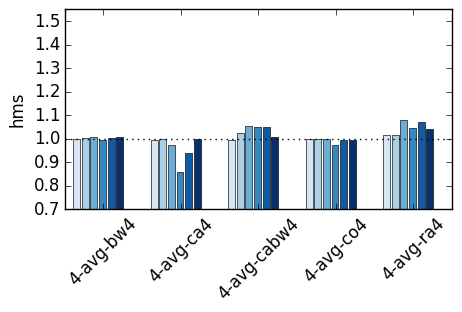
\includegraphics[width=\textwidth]{figures/results/speedup/avg-hms-0128k-0100-4-avg}
        \caption{HMS}
        \label{fig:results:base:4-avg:hms}
    \end{subfigure}
    \begin{subfigure}[b]{0.5\textwidth}
        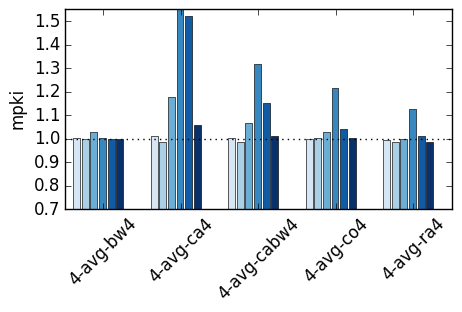
\includegraphics[width=\textwidth]{figures/results/speedup/avg-mpki-0128k-0100-4-avg}
        \caption{MPKI (not shown ca4 pipp 1.9)}
        \label{fig:results:base:4-avg:mpki}
    \end{subfigure}
    \caption[Average result for 4-core workloads]{Average \gls{stp}, \gls{hms} and \gls{mpki} normalized to \gls{lru} for all 4-core workload groups.}
    \label{fig:results:base:4-avg} 
\end{figure}

Our 4-core workloads consist of five distinct groups, where four of the groups contain benchmarks with a specific characteristic.
Section~\ref{sec:methodology:benchmarks} lists each group and explain their specific characteristics.
Figure~\ref{fig:results:base:4-avg} shows average \gls{stp}, \gls{hms} and \gls{mpki} normalized to \gls{lru} for these five groups.
Exploring the result from each of these groups individually is useful as it will show how various algorithms react to specific workload characteristics.

Bandwidth bound workloads contain benchmarks that do not benefit from increased cache space.
These are benchmarks with mainly streaming access patterns. 
As expected the results show that none of the algorithms can significantly improve performance compared to \gls{lru}.
As seen in Figure~\ref{fig:results:base:4-avg:mpki} \gls{ucp} causes 3\% more misses than \gls{lru}, and in return increases \gls{stp} by 4.8\% compared to \gls{lru}.
We expect that even our bandwidth bound benchmarks will have phases with memory re-references, which means that their utility will increase.
Based on our results, \gls{ucp} seems to detect these phases and prioritize benchmarks correctly.
While \gls{pipp} in theory also should be able to detect such changes, our result shows it does not.
A possible explanation to this is that \gls{pipp} uses both utility and streaming flags.
While an application may periodically have increased utility causing \gls{ucp} to prioritize it, \gls{pipp} might still consider it as streaming due to a high miss-fraction, if this is the case, \gls{pipp} will ignore the increased utility.

Cache bound workloads contain benchmarks that are sensitive to changes in available cache space.
In general these benchmarks have recency-friendly access patterns.
Our results from these workloads show two main trends.
First, as expected, \gls{lru} performs well, and none of the other algorithms increases performance or significantly reduce misses.
Secondly, \gls{ucp} and \gls{pipp}, the two algorithms that perform way partitioning, both reduce performance and cause a significant miss increase. 
While \gls{tadip} and \gls{drrip}, which both mimic \gls{lru} and \gls{prism}, which performs a variant of block level partitioning, performs as good as \gls{lru} in terms of performance.
From this, we see that way partitioning is not beneficial if all benchmarks are recency-friendly.
This is an expected result, as way-partitioning is designed to improve performance by shielding recency-friendly access patterns from thrashing caused by other cores.
When all applications are recency-friendly, it seems that having the cores dynamically share the cache based on access frequency is a better solution.
\gls{prism}, which does block level partitioning, confirms this assumption as it performs as good as \gls{lru} in terms of \gls{stp} and \gls{hms}.
It does, however, cause a small increase in misses.

The performance of compute-bound workloads is expected to be mostly unaffected by the partitioning algorithm. 
Our results support this assumption, with the exception of PIPP, which again causes increased misses and a slight performance decrease.
Once again, PIPP-min8 seems to remedy this, pointing to an issue with short block lifetimes in a PIPP managed cache, causing more misses.

Both cache and bandwidth bound workloads and the random workloads show results that concur with the overall averages discussed earlier.
One interesting fact to note is that both versions of PIPP and UCP are equally good and also the best performers when measuring in HMS in cache and bandwidth bound workloads.
This result points to PIPP being able to provide speedups of individual benchmarks that are good enough to raise the average while still performing as good as LRU measured in STP.
Most likely this indicates that applications marked as streaming are performing badly while those shielded are performing so good their performance increase raises the average.


\section{Cache- And Bandwidth-Bound Workload Results}
\begin{figure}[th]
    \centering
    \begin{subfigure}[b]{0.5\textwidth}
        \includegraphics[width=\textwidth]{figures/results/speedup/speedup-stp-0128k-0100-cabw4}
        \caption{STP}
        \label{fig:results:base:cabw:stp}
    \end{subfigure}%
    \begin{subfigure}[b]{0.5\textwidth}
        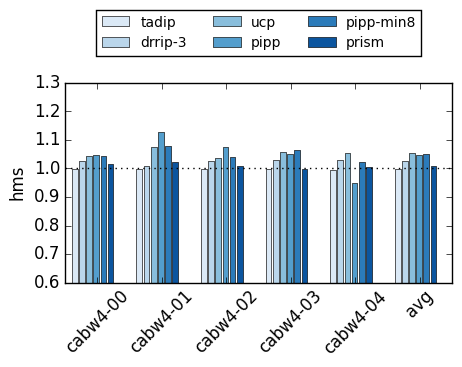
\includegraphics[width=\textwidth]{figures/results/speedup/speedup-hms-0128k-0100-cabw4}
        \caption{MPKI}
        \label{fig:results:base:cabw:mpki}
    \end{subfigure}
    \caption[cabw workloads result]{STP and \gls{mpki} normalized to \gls{lru} for cache and bandwidth bound workloads.}
    \label{fig:results:base:cabw} 
\end{figure}

In all our previous findings, we have observed that UCP is raising performance while also increasing misses.
To ensure that this result is not just an artifact of result averaging, we show the per workload STP and MPKI for the cache and bandwidth bound workloads in Figure~\ref{fig:results:base:cabw}.
As expected, the STP measurements show UCP providing a speedup in four out of five workloads.
In the fifth workload, cabw01, UCP performs as good as LRU.
When considering the MPKI measurements, we observe that UCP increase misses by at least 30\% in the four workloads where performance is best.
We also note that in the case where UCP performs as good as LRU, it also causes the least number of misses.
These same trends are also visible in our other results.
Based on this, we conclude that \gls{ucp} can increase performance while also increasing misses.